% Plot Hochpass
% Minimalistisch (sketch-like for beamer presentation)
% Amplitudengang
% plots with same width for vertical alignment:
%   plot_tiefpass_mini_ampli_lin_samesize.tex
%   plot_tiefpass_mini_phase_lin_samesize.tex
%   plot_hochpass_mini_ampli_lin_samesize.tex
%   plot_hochpass_mini_phase_lin_samesize.tex
% TODO: Alignment via invisible boundbox
\def\ttau{0.01}%                % Zeitkonstante tau = 0.01 s 
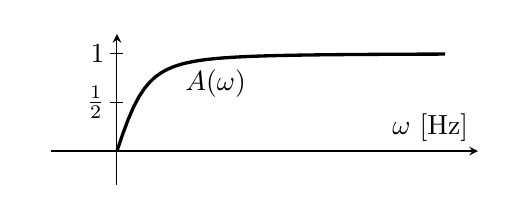
\begin{tikzpicture}%
    % invisible boundbox
    \draw[draw=none](-0.3,-0.125) rectangle (+5.5,+2); % bbox % set draw=black (debug) or draw=none (final)
\begin{axis}[%
    xlabel={$\omega\ [\mathrm{Hz}]$},
    xmin=-200, xmax=1100,       % alignment solution with x-axis (bigger than y-labels):
    domain=1:1000, 
    ymin=-0.35, ymax=1.2,
    samples=61,
    axis x line=center,
    axis y line=center,
    width=7cm,
    height=3.5cm,
    ticks=none,                 % own ticks, otherwise rescaling and no alighnment with other plot
]   % A(omega) = 1/(1+1/(omega*tau)^2)^0.5
    \addplot[mark=none,very thick,]{1/(1+1/(x*\ttau)^2)^0.5}  node[pos=0.3,anchor=north] {$A(\omega)$};%plot + plotlabel
    \addplot[black,thin] coordinates{(-20,0.5)(+20,0.5)}    node[anchor=east,black] {$\frac{1}{2}\ $};% yaxis tick
    \addplot[black,thin] coordinates{(-20,1)(+20,1)}        node[anchor=east,black] {$1\ $};% 			yaxis tick
\end{axis}%
\end{tikzpicture}% Keine Leerzeichen danach!